\documentclass[11pt,a4paper]{article}
\usepackage[utf8]{inputenc}
\usepackage[T1]{fontenc}
\usepackage{amsfonts}
\usepackage[french]{babel}
\frenchbsetup{StandardLists=true} % à inclure si on utilise \usepackage[francais]{babel}
\usepackage{enumitem}
\usepackage{amssymb}
\usepackage{amsmath}
\usepackage[left=2cm,right=2cm,top=2cm,bottom=2cm]{geometry}
\usepackage{multirow}
\usepackage[dvipsnames]{xcolor}

\usepackage[T1]{fontenc}
\usepackage{graphicx}

\usepackage{setspace}
\singlespacing

\usepackage{pstricks}
\usepackage{xkeyval}
\usepackage{pst-labo}


\usepackage{multicol}
\usepackage{caption}
\usepackage{fancyhdr}
\pagestyle{fancy}
\renewcommand\headrulewidth{1pt}
\fancyhead[L]{Lycée Denis Diderot }
\fancyhead[R]{Classe de 1 Bac Pro }
\setcounter{page}{3}\fancyfoot[C]{page \thepage}
\fancyfoot[R]{Année 2024-2025}
\fancyfoot[L]{Alexis RUIZ}
\usepackage{multirow,tabularx,booktabs}
\usepackage[tikz]{bclogo} 
\usepackage{circuitikz}

\newcommand{\cadreblanc}[1]{%
\medskip\framebox[\linewidth][c]{%
\rule{0mm}{#1mm}}\par
\medskip}

\usepackage{awesomebox}
\setlength{\aweboxvskip}{0mm}
\usepackage{pifont}
\usepackage{chemmacros}
\chemsetup{modules=all}
\setlength{\columnseprule}{.25mm}

\renewcommand{\arraystretch}{2}
\newcommand*\acocher{\quitvmode{\fboxsep0pt \fboxrule0.8pt \fbox{\vrule height1.8ex depth.1ex width0pt \vrule height0pt depth0pt width1.9ex }}}

\newcolumntype{C}[1]{>{\centering\arraybackslash }b{#1}}

\newcommand{\code}{\awesomebox[black]{2pt}{

\includegraphics[scale=0.15]{../Chapitre 1 - Energie et puissance électrique/images/frame.png}
}{black}}

\newcommand{\moteur}{\awesomebox[black]{2pt}{

\includegraphics[scale=1]{images/moteur.jpg} 
}{black}}

\newcommand{\defbox}{\awesomebox[black]{2pt}{
\includegraphics[scale=0.5]{images/appel exam.png}}{black}}

\newcommand{\defconclusion}{\awesomebox[black]{2pt}{\rotatebox{90}{\Large{\textbf{Conclusion}}}}{black}}

  \newenvironment{itemize*}%  % listes compactes
    {\begin{itemize}%
      \setlength{\itemsep}{0pt}%
      \setlength{\parskip}{0pt}}%
    {\end{itemize}}

\frenchbsetup{StandardLists=true}



\begin{document}


\flushleft \textbf{NOM : \hfill Classe : \hspace{3cm} ~~\\[2mm]
Prénom:\\[0,4cm]
}
\hrule\
\\[0,2cm]

\begin{center}
 \LARGE{TP1 - Comment évolue la pression en fonction du volume ? }
\end{center}

\vspace{3 mm}

\normalsize

\hrule\
\\[0,2cm]
   \begin{center}
   \textbf{Le soin et la rédaction interviendront dans la notation.}
   \end{center} 

\vspace{4mm}



\fcolorbox{black}{white}{\textbf{1. Expérience}}  \\[3mm]
 \begin{enumerate}[label*=1.\arabic*.]
 	
\item 

\noindent%
\begin{minipage}{.4\textwidth}%
 \begin{bclogo}[couleur=white ,  arrondi =0.1 , logo = \bcinfo, epBarre =2]{ Matériel }

\begin{itemize*}
    \item 1 seringue de 100 mL graduée tous les 10 mL.
    \item 1 tuyaux souple de 3mL
    \item 1 boitier capteur de pression
    \item 1 ordinateur avec python installé
\end{itemize*}
\end{bclogo}

\end{minipage}%
\hfill
\begin{minipage}{.5\textwidth}%

\begin{center}
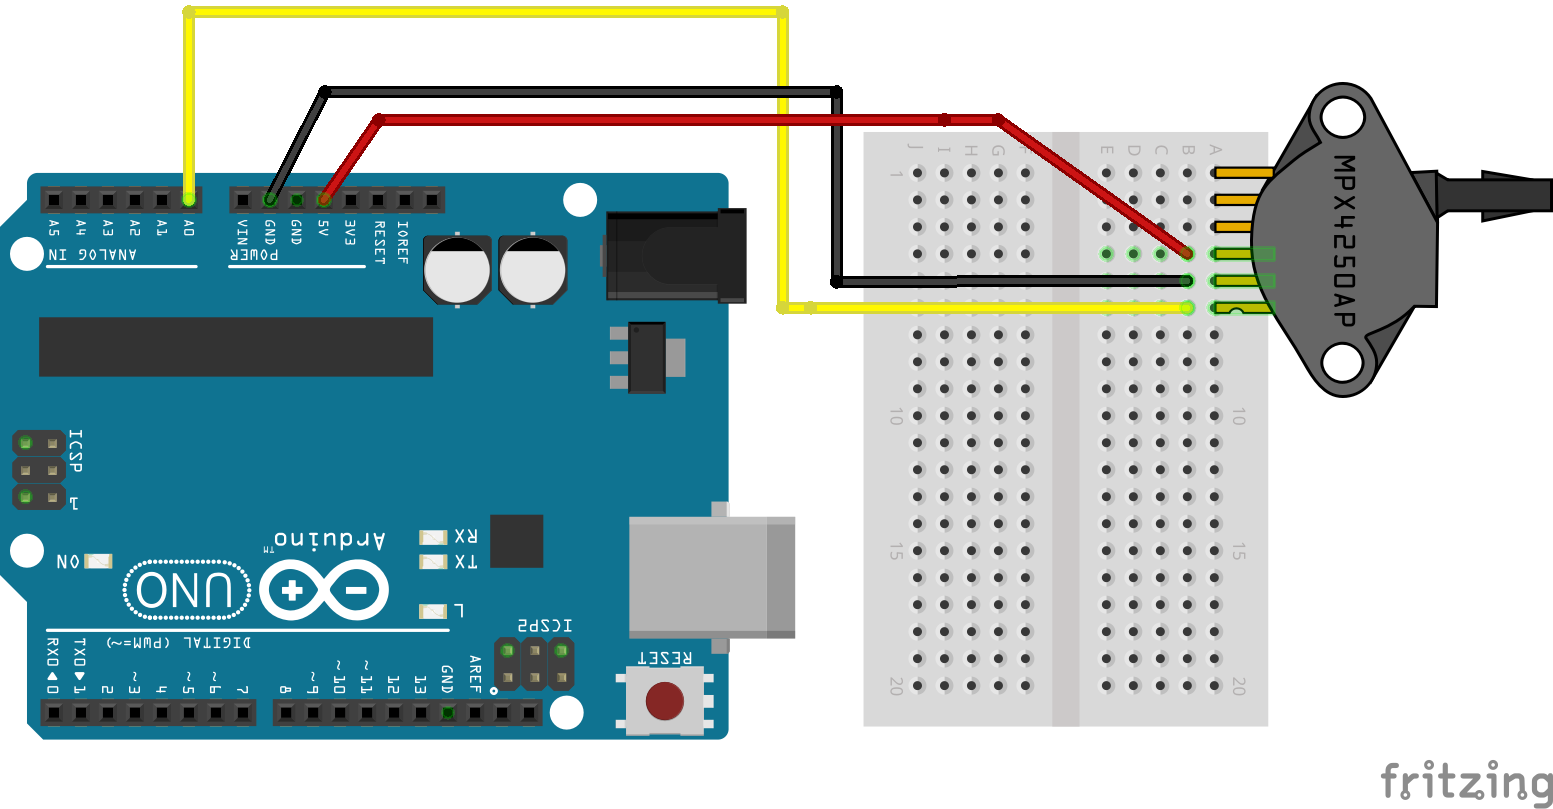
\includegraphics[width=\textwidth]{images/capteurpression.png}
 
\end{center}
\end{minipage}%

Il suffit de raccorder l'extrémité de la seringue au tuyau souple du capteur de pression comme sur la photo ci-dessus, puis le boîtier de mesures à l'ordinateur à l'aide du câble USB.

Aller dans le répertoire de votre classe, dans le dossier Sciences physiques, ouvrir le fichier mariotte.exe. Appuyer sur F11 pour être en plein écran. 


On veut mesurer la pression en fonction du volume occupé par le gaz dans la seringue. \\ Pour cela, on fera une série de 9 mesures pour des volumes compris entre  de 20 cm$^3$ à 60 cm$^3$, la pression correspondante sera enregistrée par le logiciel. 

\vfill 
    
\defbox{\fbox{
\begin{minipage}{8cm}{

Appeler M Ruiz pour qu'il vérifie le montage.}

\end{minipage}
}}

\vfill

\item Mesures : 

\begin{itemize}
    \item Tourner le sélecteur au bout de la seringue vers la gauche.
    \item Placer le piston de la seringue sur 40 cm$^3$
    \item Tourner le sélecteur au bout de la seringue vers la haut.
    \item Dans la partie "Volume de gaz", cliquez sur le bouton 40 puis cliquer sur ajouter mesure. le logiciel attendra la stabilisation, puis un point s'affichera dans chacun des graphiques. 

    \vfill 
    
\defbox{\fbox{
\begin{minipage}{8cm}{

Appeler M Ruiz pour qu'il vérifie le montage.}

\end{minipage}
}}

\item effectuer toutes les mesures proposées entre 35 cm$^3$ et 20 cm$^3$ en compression, la pression doit augmenter. 
\item effectuer toutes les mesures proposées entre 45 cm$^3$ et 60 cm$^3$ en détente, la pression doit diminuer. 
\item Ouvrir l'onglet tableur (en haut des graphiques) 

\end{itemize}

\end{enumerate}

\newpage

\fcolorbox{black}{white}{\textbf{2.Résultats}}  \\[3mm]




\begin{center}
\begin{tabular}{|p{1.8cm}|*{9}{C{1.0cm}|}}
\hline
$V$ (cm$^3$)    & 20 & 25 & 30 & 35 & 40 & 45 & 50 & 55 & 60 \\
\hline
$P$ (kPa)       &    &    &    &    &    &    &    &    &    \\
\hline
$P \times V$    &    &    &    &    &    &    &    &    &    \\
\hline
\end{tabular}
\end{center}



\fcolorbox{black}{white}{\textbf{3. Exploitation}}  \\[3mm]

\begin{enumerate}[label*=3.\arabic*.]

	\item Commenter les résultats du produit p$\times$V. \\[8mm]
	
	\dotfill
	
	\vspace{5mm}
	On veut modéliser $p=f(V)$ : \\[3mm]

	
	
	\item Cliquer sur l'onglet modélisation automatique et saisir pm = constante/V dans le champ de texte correspondant.
	
	\item Cliquer ensuite sur Modéliser et relever la valeur de la constante. \\[8mm]
	
	\dotfill 
	
	\vfill 
	
	
	\defbox{\fbox{
			\begin{minipage}{9cm}{
					
					Appeler M Ruiz pour qu'il vérifie vos résultats.}
				
			\end{minipage}
	}}
	
	\vfill 
	
	\end{itemize}
	
	\vfill 
	
	\fcolorbox{black}{white}{\textbf{3. Exploitation}}  \\[3mm]
	
	\begin{itemize}
	\item 
	
	
	Quel type de courbe obtient-on ? \\[3mm]
	
	\dotfill 
	
	Comment évoluent les grandeurs pression et volume au cours de cette expérience ? \\[3mm]
	
	\dotfill 
	
	\vspace{3mm}
	
	\dotfill 
	
	
	
	\item Parmi ces affirmations, cocher celles qui sont justes : \\[3mm]
	
	\begin{itemize}[label=$\square$]
		
		
		\item A température constante, quand la pression d'un gaz augmente, son volume augmente. 
		
		\item A température constante, le volume d'un gaz et sa pression sont des grandeurs       proportionnelles. 
		
		\item A température constante, le volume d’un gaz est inversement proportionnel à la pression        qu’il reçoit. 
		
		\item A température constante, la pression d'un gaz évolue en fonction du carré de son volume. 
		
	\end{itemize}
	\end{itemize}
	
	\dotfill
	
%\end{enumerate}

\end{document}